\documentclass[oneside]{jgeccse}

%%% Macro definitions for Commonly used symbols
\newcommand{\Rey}{\ensuremath{\mathrm{Re}}}
\newcommand{\avg}[1]{\ensuremath{\overline{#1}}}
\newcommand{\tenpow}[1]{\ensuremath{\times 10^{#1}}}
\newcommand{\pder}[2]{\ensuremath{\frac{\partial#1}{\partial#2}}}

% Referencing macros
\newcommand{\Eqref}[1]{Equation~\eqref{#1}}
\newcommand{\Tabref}[1]{Table~\ref{#1}}
\newcommand{\Figref}[1]{Figure~\ref{#1}}
\newcommand{\Appref}[1]{Appendix~\ref{#1}}

\usepackage{longtable} % allows the literature-review table to break across pages

\graphicspath{{Images/}}

\begin{document}
	
%%********************************Frontmatter***********************
% In frontmatter everything comes with roman numbering	
\pagenumbering{roman}
\setcounter{page}{1}

%*******************************************************************
%                         Title Page                            
%*******************************************************************
\title{TimberTrace: A Blockchain-Based Provenance Tracking System for Teakwood} % Project title
%%%
\firstauthor{Sauparna Gupta } %Capitalize first letter of each word of students' name
\firstrollnumber{Intern ID } % Roll Number
\secondauthor{Sanjay Sarkar} %Capitalize first letter of each word of students' name
\secondrollnumber{Intern ID }% Roll Number
\thirdauthor{Chayan Barman} %Capitalize first letter of each word of students' name
\thirdrollnumber{Intern ID } % Roll Number
%\forthauthor{Forth Author Name}  %Comment/remove this line if 4th candidate is not in the group
%\forthrollnumber{Scholar ID4}

%% Project Group ID
%\groupid{MJP18XX} %Mention your group ID here 

%% Print the date. Today's date comes by default, change it here to 
%% other date format, if required:

\date{\today}
%\date{10 May 2020}


%% The type of the report can be set here

\reporttype{Project Report}

%% Name of the degree
\degree{Bachelor of Technology}


%% Department/Centre Name
\dept{Computer Science and Engineering}


\supervisor{Dr. Subhas Barman\\
Assistant Professor \& Head }  % Guide name
%\cosupervisor{Assistant Professor \& Head } % Designation
%\excosupervisor{External Supervisor}



\maketitle

%*******************************************************************
%                         Dedication Page                         
%*******************************************************************
%\dedication[Dedicated to \ldots]        
%\addintoc{Dedication}


%*******************************************************************
%                        Certificate Page                         
%*******************************************************************
\makecertificate[Certificate]{project report}
%\addintoc{Certificate}

%*******************************************************************
%                          Declaration                           
%*******************************************************************
%==================================dec.tex================================
%
\begin{Declaration}
\begin{flushright}
JGEC Jalpaiguri\\
 \today
\end{flushright}
\vspace*{0.5cm}

\noindent
We declare that this written submission represents our ideas in our own words and where others' ideas or words have been included, We have adequately cited and referenced the original sources. We declare that We have properly and accurately acknowledged all sources used in the production of this report. We also declare that We have adhered to all principles of academic honesty and integrity and have not misrepresented or fabricated or falsified any idea/data/fact/source in our submission. We understand that any violation of the above will be a cause for disciplinary action by the Institute and can also evoke penal action from the sources which have thus not been properly cited or from whom proper permission has not been taken when needed. 

\DecSign

%
\end{Declaration}
%========================================================================
















 
%\addintoc{Declaration}

%*******************************************************************
%                        Acknowledgements                    
%******************************************************************* 
%%%
\acknowledgments
\begin{flushright}
JGEC Jalpaiguri \\
 \today
\end{flushright}
\vspace*{0.5cm}

This section is for the acknowledgments. Please keep this brief and resist the temptation of writing flowery prose! Do include all those who helped you, e.g. other faculty/staff you consulted, colleagues who assisted etc.



\signature

%========================================================================

%%% Local Variables: 
%%% mode: latex
%%% TeX-master: "../mainrep"
%%% End:  


%******************************************************************
%                          Abstract                             
%******************************************************************  
%============================= abstract.tex================================
\begin{Abstract}
This report proposes a blockchain-based solution to the challenges faced by traditional e-voting systems, such as security, transparency, and trust. The proposed system allows voters to cast their votes remotely from their computer or mobile device. The voters have no need to visit a polling booth physically for casting their vote. In this project, voter authentication is carried out by UIDAI's Aadhar authentication, the system ensures that each voter can only cast one vote and that their votes remain anonymous. In the implementation, the smart contract is developed in Solidity and deployed to execute the e-voting system on the Ethereum blockchain. The results of the proposed system are compared to state-of-the-art methods, demonstrating the feasibility and potential of this technology in revolutionizing the voting process. 
\noindent Keywords: E-voting systems,Ethereum blockchain, Voter authentication, Smart contract
%
%
%
%
%
\end{Abstract}
%=======================================================================

                    

%******************************************************************
%                         Contents list                         
%******************************************************************
%\figurespagefalse
%\tablespagefalse
\makecontents % Creats toc, lof, and lot

%******************************************************************
%                        Notations                              
%******************************************************************
\notations[4cm]{List of Symbols}      

%%********************************Mainmatter***********************
% In mainmatter everything comes with arabic numbering	
\cleardoublepage
\setcounter{page}{1}
\pagenumbering{arabic}

%******************************************************************
%                         Chapters                           
%****************************************************************** 
\include{Chapters/ch1-Introduction}
\chapter{Literature Review}
\label{ch2-LiteratureReview}

Using blockchain to trace goods through a supply chain is not a new idea.
Over the last few years researchers have tried it in a number of areas,
from food and medicine to forestry and factory manufacturing. We went
through ten of these earlier works before we started building
\emph{TimberTrace}. Some are published research papers and some are
open-source projects that other developers have put on GitHub. We did not
just read them for background; in each one we looked for a particular idea
worth borrowing. Sometimes we used the idea more or less as it was, other
times we changed it to fit timber, and in a few cases we decided a simpler
option made more sense for a student prototype. The rest of this chapter
goes through these works one by one and points out exactly which design
choice in our own project each of them shaped.

\section{Survey of Related Work}

The work closest to ours is by Figorilli et al.~\cite{figorilli2018wood}.
As far as we know, it was the first published attempt to trace wood
electronically across the whole supply chain using a blockchain. They put
RFID tags on the logs and wrote each scan to an immutable ledger, so the
physical wood and its digital record stayed linked. Westerkamp et
al.~\cite{westerkamp2018token} looked at the problem from a different
angle. In their ``token-recipe'' model, making a product means using up
the tokens that stand for its raw materials and creating a new token for
the finished item, which keeps the link between inputs and outputs on the
chain itself. Two more projects helped shape the consumer-facing side of
our work: the SCTS system~\cite{scts} let anyone check a product's history
by scanning a QR code, and the \verb|trace| dApp~\cite{trace} went a step
further by attaching signed certificates from trusted experts to each
product. A third, \verb|smart-traceability|~\cite{smarttraceability},
showed a neat way to handle large files by keeping the batch data on IPFS
and storing only its hash on-chain.

A second group of works deals mainly with who is allowed to do what.
PharmaChain~\cite{pharmachain} and the dual-contract design in
Ref.~\cite{dualcontract} both handle roles carefully; the latter even
splits the data and the permission logic into separate contracts so the
rules can be updated without disturbing the stored records. The dApp in
Ref.~\cite{faizack} treats the supply chain as a set of fixed stages that
a product can only move forward through, with role checks guarding each
step. Finally, two studies made us think harder about which blockchain to
build on. The Hyperledger Fabric system in Ref.~\cite{hyperledger} showed
what a permissioned, enterprise-grade network can do, and the recent
timber-focused framework in Ref.~\cite{timberSC2025} added something we
had overlooked, treating the transfer of ownership as its own recorded
action on the chain rather than just another event.

\section{Comparative Summary}

Table~\ref{tab:litreview} consolidates the survey, listing each
paper/project alongside the specific idea we carried into
\emph{TimberTrace}.

\renewcommand{\arraystretch}{1.35}
\begin{longtable}{|c|p{5.1cm}|p{6.6cm}|}
  \caption{Literature reviewed and the idea adopted in this project.}
  \label{tab:litreview} \\
  \hline
  \textbf{Sl.\ No.} & \textbf{Paper / Project Name} & \textbf{Idea Used in My Project} \\
  \hline
  \endfirsthead

  \multicolumn{3}{c}%
  {\tablename\ \thetable\ -- \textit{continued from previous page}} \\
  \hline
  \textbf{Sl.\ No.} & \textbf{Paper / Project Name} & \textbf{Idea Used in My Project} \\
  \hline
  \endhead

  \hline
  \multicolumn{3}{r}{\textit{continued on next page}} \\
  \endfoot

  \hline
  \endlastfoot

  1 & Figorilli et al. (2018), ``A Blockchain Implementation Prototype
  for the Electronic Open Source Traceability of Wood along the Whole
  Supply Chain,'' \emph{Sensors}, MDPI~\cite{figorilli2018wood} &
  Recording every physical handoff of the wood (harvest $\rightarrow$
  lot $\rightarrow$ batch $\rightarrow$ furniture) as an immutable,
  tamper-proof on-chain event, so the ledger is a permanent provenance
  record of each stage. \\
  \hline

  2 & Westerkamp, Victor \& K\"upper (2018), ``Blockchain-based Supply
  Chain Traceability: Token Recipes Model Manufacturing
  Processes,'' IEEE Blockchain~\cite{westerkamp2018token} &
  The input-consumed-to-output manufacturing model, realised as our
  UTXO-inspired mass-balance rule in which a Lot is consumed to create a
  Batch and a Batch to create Furniture, preserving the input--output
  link on-chain. \\
  \hline

  3 & SCTS --- Supply Chain Tracking System (AtrauraBlockchain,
  GitHub)~\cite{scts} &
  Placing a QR code on the physical product that resolves its full
  on-chain history, enabling anyone to audit provenance without special
  access --- our \texttt{/verify} QR flow. \\
  \hline

  4 & \texttt{maximevaillancourt/trace} --- certification dApp
  (GitHub)~\cite{trace} &
  Attaching signed certificates to products; we store a certificate
  IPFS CID inside the Lot and Furniture records as a lightweight
  certification layer over the provenance data. \\
  \hline

  5 & \texttt{ecobioca/smart-traceability} (GitHub)~\cite{smarttraceability} &
  Storing all bulky batch/product metadata (certificates, product
  images) off-chain on IPFS via Pinata and keeping only the content
  hash on-chain to save storage and gas. \\
  \hline

  6 & PharmaChain (Bapatla et al., 2022), \emph{IET
  Networks}~\cite{pharmachain} &
  Role-based access control enforced through Solidity function
  modifiers --- our \texttt{AUCTION\_HOUSE\_ROLE} and
  \texttt{FACTORY\_ROLE} guarded by OpenZeppelin's
  \texttt{onlyRole()}, with the admin granting/revoking roles. \\
  \hline

  7 & Dual-Contract Architecture with RBAC (2025), \emph{Scientific
  Reports}~\cite{dualcontract} &
  Separation of concerns between authoritative logic and data ---
  reflected in our decoupling of the authoritative smart contract (source
  of truth) from the read-optimised PostgreSQL mirror, and noted as a
  future dual-contract upgrade path. \\
  \hline

  8 & \texttt{faizack/Supply-Chain-Blockchain} (GitHub)~\cite{faizack} &
  Modelling the supply chain as defined, role-gated stages with a
  dedicated contract function for each transition
  (\texttt{registerLot}, \texttt{purchaseWood},
  \texttt{createFurniture}). \\
  \hline

  9 & High-Efficiency Blockchain-Based Supply Chain Traceability
  (Hyperledger Fabric, 2022)~\cite{hyperledger} &
  Throughput comparison of permissioned vs.\ public ledgers, which
  informed our deliberate choice of public Ethereum Sepolia for the
  prototype and identified Hyperledger as the future scaling path. \\
  \hline

  10 & Blockchain-Enabled Smart Contracts for Secure Timber
  Traceability (2025), ScienceDirect~\cite{timberSC2025} &
  On-chain ownership tracking (the \texttt{owner} field on each Lot,
  Batch and Furniture) together with QR-based consumer verification of
  the harvested-and-certified timber. \\
  \hline

\end{longtable}
\renewcommand{\arraystretch}{1.0}

\section{Research Gap}

Across the surveyed works, three consistent trade-offs emerge. First,
hardware-driven systems~\cite{figorilli2018wood} achieve automation at the
cost of expensive IoT infrastructure, whereas a software-only,
operator-signed model is more appropriate for a research prototype.
Second, token-heavy representations~\cite{westerkamp2018token,
smarttraceability} and per-product contracts~\cite{scts} offer flexibility
but at higher gas cost and reduced auditability compared with a single
monolithic contract using struct linkage. Third, enterprise permissioned
ledgers~\cite{hyperledger} provide superior throughput but demand
self-operated infrastructure. \emph{TimberTrace} occupies the gap between
these extremes: a software-only, single-contract Ethereum system that
enforces a mass-balance conservation invariant on-chain, mirrors state to
a fast read database off-chain, and exposes QR-based public verification
--- combining the most relevant ideas from the literature into a
lightweight, auditable timber-provenance prototype.


%%% Local Variables:
%%% mode: latex
%%% TeX-master: "../mainrep"
%%% End:


\chapter{Problem Formulation and Proposed Solution}

\section{Figures and Tables}

Figures are conveniently included using postscript format.  If you are
generating a figure in a software, please check if the software
supports writing to a postscript or a PDF format. This format is loss
less vector format and with reproduce in any magnification without any
pixelation. Make sure to write it to an ``Encapsulated Post-script''or
.eps format.


\begin{figure}[!htbp]
  \centering
   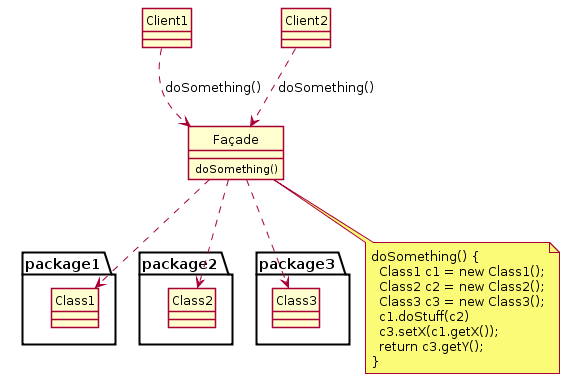
\includegraphics[width=0.65\textwidth]{Fig1}
    \caption[UML Class diagram]{UML Class diagram showing an example of the Facade design pattern. The caption of the figure goes here. A shorter caption can be written in square brackets to identify it in the list of figures if required.}
    \label{fig:1} 
\end{figure}

Figures should be given a label and which can be used to refer to them
in the running text using \verb|\ref{}| command. Figure~\ref{fig:1}
describes the process flow sheet of the Facade design pattern used in
this study. 
Two simple graphs are shown in Figure~\ref{fig:2}. 
Multiple figures with same caption can be arranged as shown in Figure~\ref{fig:2} and they are referred in text such as Figure~\ref{fig:2a} and Figure~\ref{fig:2b}. The graphs should be drawn at appropriate places with center alignment and it should be referred in text.

\begin{figure}[!htbp]
     \centering
     \begin{subfigure}{0.45\textwidth}
         \centering
         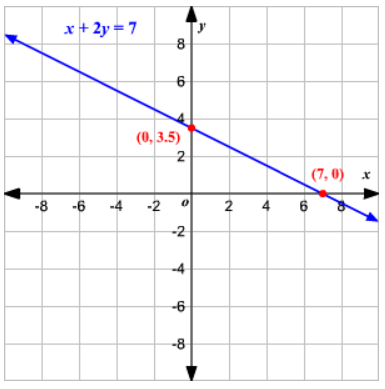
\includegraphics[width=\textwidth]{Fig2a}
         \caption{Figure2a}
         \label{fig:2a}
     \end{subfigure}
     \hfill
     \begin{subfigure}{0.45\textwidth}
         \centering
         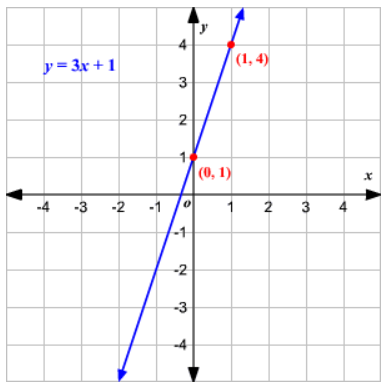
\includegraphics[width=\textwidth]{Fig2b}
         \caption{Figure2b}
         \label{fig:2b}
     \end{subfigure}
        \caption{Two simple graphs}
        \label{fig:2}
\end{figure}


The format for tables is given below. The table must referred in
the text as Table~\ref{tab:1}. The title of the table with table number should be written at the top of the table with center aligned as shown below in Table~\ref{tab:1}.

\begin{table}[!htbp]
    \centering
    \caption{A table shows an example of multirow and multicolumn.}
    \label{tab:1}
\begin{tabular}{|l|l|l|l|}\hline
  \multirow{10}{*}{numeric literals} & \multirow{5}{*}{integers} & in decimal & \verb|8743| \\ \cline{3-4}
  & & \multirow{1}{*}{in octal} & \verb|0o7464| \\ \cline{2-4}
  & & \multirow{2}{*}{in hexadecimal} & \verb|0x5A0FF| \\ \cline{4-4}
  & & & \verb|0xE0F2| \\ \cline{2-4}
  & \multirow{4}{*}{fractionals} & \multirow{4}{*}{in decimal} & \verb|140.58| \\ \cline{4-4}
  & & & \verb|8.04e7| \\ \cline{4-4}
  & & & \verb|0.347E+12| \\ \cline{4-4}
  & & & \verb|47e22| \\ \cline{1-4}
  \multicolumn{3}{|l|}{\multirow{3}{*}{char literals}} & \verb|`H'| \\ \cline{4-4}
  \multicolumn{3}{|l|}{} & \verb|`\n'| \\ \cline{4-4}          %% here
  \multicolumn{3}{|l|}{} & \verb|`\x65'| \\ \cline{1-4}        %% here
  \multicolumn{3}{|l|}{\multirow{2}{*}{string literals}} & \verb|``bom dia"| \\ \cline{4-4}
  \multicolumn{3}{|l|}{} & \verb|``ouro preto\nmg"| \\ \cline{1-4}          %% here
\end{tabular}
\end{table}

A simple table is shown in Table~\ref{tab:2}. One may use the online latex table generator to get the latex code for required table: \url{https://www.tablesgenerator.com/} 

\begin{table}[!htbp]
\centering
    \caption{Simple table.}
    \label{tab:2}
    \begin{tabular}{|l|c|r|} % <-- Alignments: 1st column left, 2nd middle and 3rd right, with vertical lines in between
    \hline
      \textbf{Value 1} & \textbf{Value 2} & \textbf{Value 3}\\
      $\alpha$ & $\beta$ & $\gamma$ \\
      \hline
      1 & 1110.1 & a\\ \hline
      2 & 10.1 & b\\ \hline
      3 & 23.113231 & c\\ \hline
    \end{tabular}
\end{table}


\section{Code}

A simple JAVA code is given below:

\lstset{frame=tb,language=Java} %%% may change the language according to the code
\begin{lstlisting}
// Hello.java
import javax.swing.JApplet;
import java.awt.Graphics;

public class Hello extends JApplet {
    public void paintComponent(Graphics g) {
        g.drawString("Hello, world!", 65, 95);
    }    
}
\end{lstlisting}




%%% Local Variables: 
%%% mode: latex
%%% TeX-master: "../mainrep"
%%% End: 

%%%%%% 


\chapter{Results and Discussion}

In this chapter, ... 








\chapter{Conclusion and Future Work}

In this chapter, ... 

\section{Conclusion}

In this study, ....

\section{Future Work}

Future direction includes ....

%****************************************************************
%                         Appendices                           
%****************************************************************
%% Additional, supporting material, such as codes, derivations, etc., can be placed in the appendix
\appendix
%%%%% 

\chapter{Appendix}

\section{Appendix 1}

\section{Appendix 2}

%******************************************************************
%                         Bibliography or References          
%******************************************************************  
%\linespread{1}\selectfont
\bibliography{references}     

%*******************************************************************
%                         List of publications               
%******************************************************************
%\include{pub}            

%*******************************************************************
%                        About author                    
%*******************************************************************
%\colophon % remove this command while using this file.

% END OF THE REPORTING
%*******************************************************************
\end{document}

%%% Local Variables: 
%%% mode: latex
%%% TeX-master: t
%%% End: 
